\chapter{Results}
%\subsection{General results}
%
%After excluding faulty cameras we had TK cameras in total, 19 in the Control-group and 33 in the experiment group.
%A total of TK photos were taken, of whom TK contained photos of the species I've focused on in my study. Check table for more details.
%
%The species I've focused on was mainly night-active as displayed in the density plots \ref{fig:overlap}, (with the exception of squirrel). In other words, all of them experienced a white LED flash during night hours.
%(Caption: Figure is split up in periods with and without white LED flash. Night activity in the dashed curve highlights the times the species would have experienced the flash. "Carpet"-below the curves signifies datapoints of each "group".
%



% for results: Predicted counts visualised in \vref{fig:glmm_sp}, model parameters visualised in \vref{fig:para_sp}.


\section{GLMM}
For roe deer, the model explaining variation in detection rate has a substantial explanatory power (conditional R2 = 0.45), but the part related to the fixed effects alone (marginal R2) is just 0.01.

In other words, most of the explained variation in detection rate is due to seasonal changes and variation between the different camera sites captured in the random terms.
Neither the main effect, nor the interaction term with time were significant for the white LED periods (flash[1]).

The white LED periods had a non-significant positive effect in the beginning (flash[1] in table \ref{tab:param}) compared to the IR periods (Intercept). However, along the time since deployment-axis (time.deploy $\ast$ flash [1]) there was a negative effect, to the extent that after two months the mean detection rate was lower for white LED periods, than for IR (flash [0]; figure 3.1a). However, the confidence interval (CI) of both white LED and IR periods almost completely overlaps, and hence, are not significantly different.


As the control-group stayed unchanged through the whole study period, and was visited less than the other cameras, I expected there to be no trend over time (i.e. time.deploy $\ast$ flash [Control] $\approx 0$).
Any fluctuations in detection rates due to weekly (and ultimately seasonal) changes should be controlled for by the random effect-term for week of the year. 


% latex table generated in R 4.0.4 by xtable 1.8-4 package
% Sun Mar 14 15:22:35 2021
\begin{table}[ht]
\centering
\begin{tabular}{llllll}
  \hline
Parameter & Coefficient & SE & 95\% CI & z & p \\ 
  \hline
Roe deer &  &  &  &  &        \\ 
  (Intercept) & 0.03 & 0.01 & (0.01, 0.06) & -8.69 & $<$ .001 \\ 
  time.deploy & 0.89 & 0.05 & (0.80, 0.99) & -2.22 & 0.026  \\ 
  flash [IR] & 1.17 & 0.58 & (0.44, 3.11) & 0.31 & 0.754  \\ 
  flash [LED] & 1.24 & 0.62 & (0.47, 3.30) & 0.43 & 0.666  \\ 
  time.deploy * flash [IR] & 1.05 & 0.07 & (0.92, 1.20) & 0.69 & 0.489  \\ 
  time.deploy * flash [LED] & 1.01 & 0.06 & (0.89, 1.14) & 0.11 & 0.916  \\ 
  Red fox &  &  &  &  &        \\ 
  (Intercept) & 0.03 & 7.37e-03 & (0.02, 0.05) & -14.95 & $<$ .001 \\ 
  time.deploy & 1.00 & 0.07 & (0.88, 1.14) & -0.02 & 0.985  \\ 
  flashIR & 1.02 & 0.28 & (0.59, 1.76) & 0.07 & 0.942  \\ 
  flashLED & 1.14 & 0.32 & (0.66, 1.97) & 0.48 & 0.631  \\ 
  time.deploy:flashIR & 0.99 & 0.09 & (0.83, 1.18) & -0.06 & 0.949  \\ 
  time.deploy:flashLED & 0.97 & 0.09 & (0.82, 1.16) & -0.30 & 0.763  \\ 
  Badger &  &  &  &  &        \\ 
  (Intercept) & 0.01 & 3.90e-03 & (0.01, 0.02) & -12.45 & $<$ .001 \\ 
  time.deploy & 1.17 & 0.09 & (0.99, 1.37) & 1.90 & 0.058  \\ 
  flashIR & 1.34 & 0.51 & (0.64, 2.82) & 0.78 & 0.433  \\ 
  flashLED & 1.42 & 0.54 & (0.68, 2.97) & 0.93 & 0.352  \\ 
  time.deploy:flashIR & 1.02 & 0.10 & (0.84, 1.23) & 0.17 & 0.865  \\ 
  time.deploy:flashLED & 1.01 & 0.10 & (0.84, 1.22) & 0.10 & 0.922  \\ 
  Moose &  &  &  &  &        \\ 
  (Intercept) & 8.94e-03 & 2.95e-03 & (0.00, 0.02) & -14.31 & $<$ .001 \\ 
  time.deploy & 1.02 & 0.11 & (0.83, 1.26) & 0.21 & 0.830  \\ 
  flashIR & 1.15 & 0.43 & (0.55, 2.40) & 0.37 & 0.715  \\ 
  flashLED & 1.35 & 0.50 & (0.65, 2.80) & 0.79 & 0.427  \\ 
  time.deploy:flashIR & 1.11 & 0.15 & (0.85, 1.46) & 0.78 & 0.433  \\ 
  time.deploy:flashLED & 0.97 & 0.13 & (0.75, 1.27) & -0.19 & 0.849  \\ 
  Red deer &  &  &  &  &        \\ 
  (Intercept) & 1.73e-03 & 1.18e-03 & (0.00, 0.01) & -9.35 & $<$ .001 \\ 
  time.deploy & 0.80 & 0.12 & (0.60, 1.06) & -1.56 & 0.119  \\ 
  flashIR & 1.38 & 1.03 & (0.32, 6.01) & 0.43 & 0.671  \\ 
  flashLED & 1.34 & 1.01 & (0.31, 5.88) & 0.39 & 0.697  \\ 
  time.deploy:flashIR & 1.16 & 0.22 & (0.80, 1.69) & 0.80 & 0.424  \\ 
  time.deploy:flashLED & 1.72 & 0.33 & (1.18, 2.51) & 2.81 & 0.005  \\ 
  Lynx &  &  &  &  &        \\ 
  (Intercept) & 7.44e-04 & 4.45e-04 & (0.00, 0.00) & -12.03 & $<$ .001 \\ 
  time.deploy & 0.61 & 0.20 & (0.32, 1.15) & -1.52 & 0.128  \\ 
  flashIR & 1.56 & 1.03 & (0.43, 5.70) & 0.67 & 0.502  \\ 
  flashLED & 2.30 & 1.50 & (0.64, 8.26) & 1.28 & 0.202  \\ 
  time.deploy:flashIR & 1.76 & 0.68 & (0.83, 3.74) & 1.48 & 0.140  \\ 
  time.deploy:flashLED & 1.81 & 0.70 & (0.85, 3.84) & 1.54 & 0.124  \\ 
  Hare &  &  &  &  &        \\ 
  (Intercept) & 0.02 & 6.39e-03 & (0.01, 0.03) & -10.23 & $<$ .001 \\ 
  time.deploy & 1.09 & 0.08 & (0.94, 1.26) & 1.13 & 0.258  \\ 
  flashIR & 1.04 & 0.50 & (0.41, 2.65) & 0.08 & 0.933  \\ 
  flashLED & 1.12 & 0.53 & (0.44, 2.84) & 0.23 & 0.819  \\ 
  time.deploy:flashIR & 0.89 & 0.08 & (0.74, 1.07) & -1.28 & 0.199  \\ 
  time.deploy:flashLED & 1.00 & 0.10 & (0.83, 1.21) & 0.02 & 0.983  \\ 
  European Pine Marten &  &  &  &  &        \\ 
  (Intercept) & 2.45e-03 & 9.01e-04 & (0.00, 0.01) & -16.34 & $<$ .001 \\ 
  time.deploy & 1.25 & 0.28 & (0.81, 1.95) & 1.01 & 0.314  \\ 
  flashIR & 3.42 & 1.38 & (1.55, 7.53) & 3.06 & 0.002  \\ 
  flashLED & 2.35 & 0.96 & (1.05, 5.23) & 2.09 & 0.037  \\ 
  time.deploy:flashIR & 0.76 & 0.19 & (0.47, 1.24) & -1.08 & 0.280  \\ 
  time.deploy:flashLED & 1.06 & 0.27 & (0.64, 1.75) & 0.22 & 0.828  \\ 
  Red squirrel &  &  &  &  &        \\ 
  (Intercept) & 4.47e-03 & 2.78e-06 & (0.00, 0.00) & -8710.74 & $<$ .001 \\ 
  time.deploy & 1.22 & 7.55e-04 & (1.21, 1.22) & 314.46 & $<$ .001 \\ 
  flashIR & 1.17 & 7.24e-04 & (1.16, 1.17) & 247.49 & $<$ .001 \\ 
  flashLED & 1.58 & 9.84e-04 & (1.58, 1.59) & 740.62 & $<$ .001 \\ 
  time.deploy:flashIR & 0.66 & 4.07e-04 & (0.66, 0.66) & -679.35 & $<$ .001 \\ 
  time.deploy:flashLED & 0.96 & 5.96e-04 & (0.96, 0.96) & -65.39 & $<$ .001 \\ 
   \hline
\end{tabular}
\end{table}

								%Caption outside the .tex-file or else it would be deleted every time I update the parameter-table
\caption[Standardised model parameters]%
{\label{tab:param} Standardised model parameters \par \small Results of generalised linear mixed effect models on detection rate of species at 53 different locations in south-eastern Norway, with three different treatment levels; period with only IR camera (flash:0), period with additional white LED camera (flash:1) and site unchanged through the whole study period (flash:Control). Random effects are location ID and week of year. Standardised parameters were obtained by fitting the model on a standardised version of the dataset. 95\% Confidence Intervals and p-values were computed using the Wald approximation.}

\end{table} % må inn og fjerne end{table} kvar gong tabellen oppdaterest!

 


\begin{figure}
		\begin{subfigure}{.5\textwidth}
		  \centering
		  	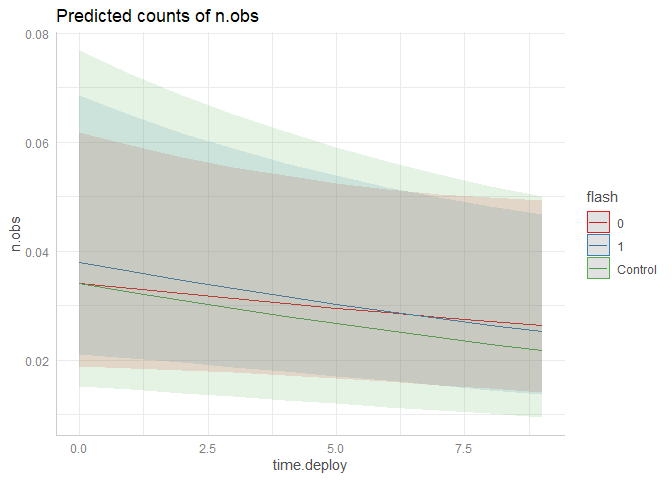
\includegraphics[width=.8\linewidth]{../R/glmm_sp_files/figure-gfm/raadyr-C-report-1.png}
		  \caption{Roe deer}
		  	\label{fig:glmm_raa}
	\end{subfigure}
		\begin{subfigure}{.5\textwidth}
		  \centering
		  	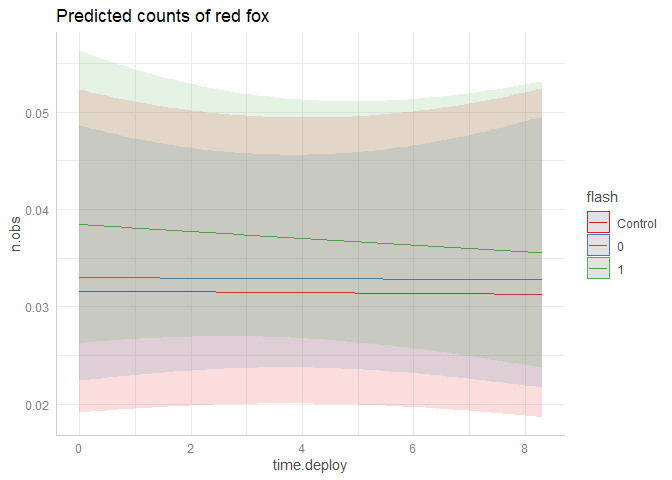
\includegraphics[width=.8\linewidth]{../R/glmm_sp_files/figure-gfm/rev-report-1.png}
		  \caption{Red fox}
		  	\label{fig:glmm_rev}
	\end{subfigure}
		\begin{subfigure}{.5\textwidth}
		  \centering
		  	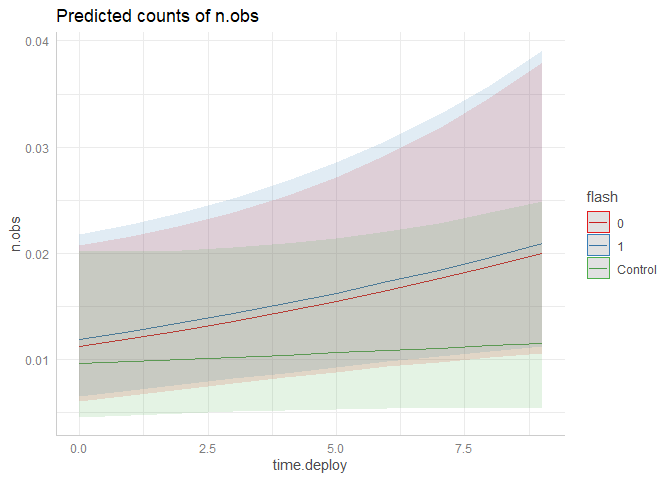
\includegraphics[width=.8\linewidth]{../R/glmm_sp_files/figure-gfm/grevling-report-1.png}
		  \caption{Badger}
		  	\label{fig:glmm_grvl}
	\end{subfigure}
		\begin{subfigure}{.5\textwidth}
		  \centering
		  	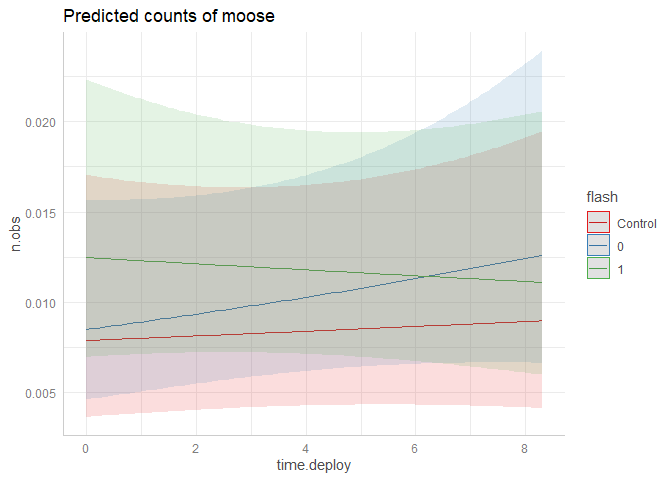
\includegraphics[width=.8\linewidth]{../R/glmm_sp_files/figure-gfm/elg-report-1.png}
		  \caption{Moose}
		  	\label{fig:glmm_elg}
	\end{subfigure}
		\begin{subfigure}{.5\textwidth}
		  \centering
		  	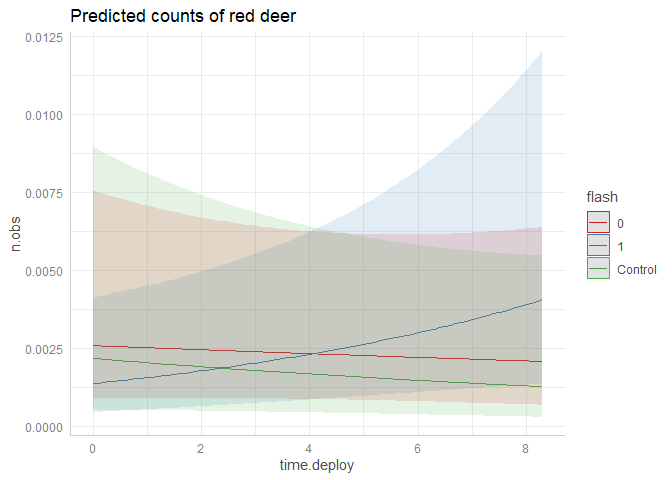
\includegraphics[width=.8\linewidth]{../R/glmm_sp_files/figure-gfm/hjort-report-1.png}
		  \caption{Red deer}
		  	\label{fig:glmm_hjort}
	\end{subfigure}
		\begin{subfigure}{.5\textwidth}
		  \centering
		  	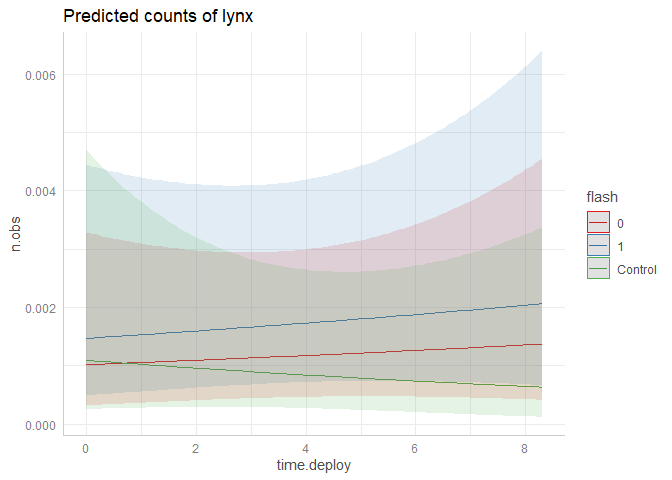
\includegraphics[width=.8\linewidth]{../R/glmm_sp_files/figure-gfm/gaupe-report-1.png}
		  \caption{Lynx}
		  	\label{fig:glmm_gaup}
	\end{subfigure}
		\caption{Fitted GLMM model to each species}
	\label{fig:glmm_sp}
\end{figure}



\begin{figure}
		\begin{subfigure}{.4\textwidth}
		  \centering
	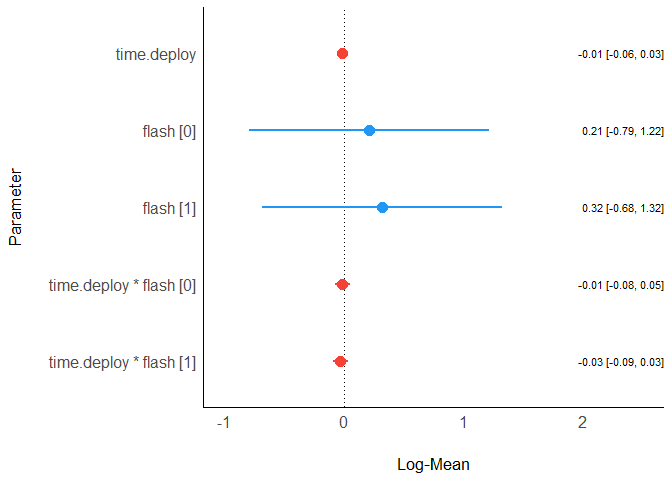
\includegraphics[scale=.4]{../R/glmm_sp_files/figure-gfm/parameters-1.png}
\caption{Intercept included}
		\label{fig:para_raa1}
	\end{subfigure}
		\begin{subfigure}{.4\textwidth}
		  \centering
	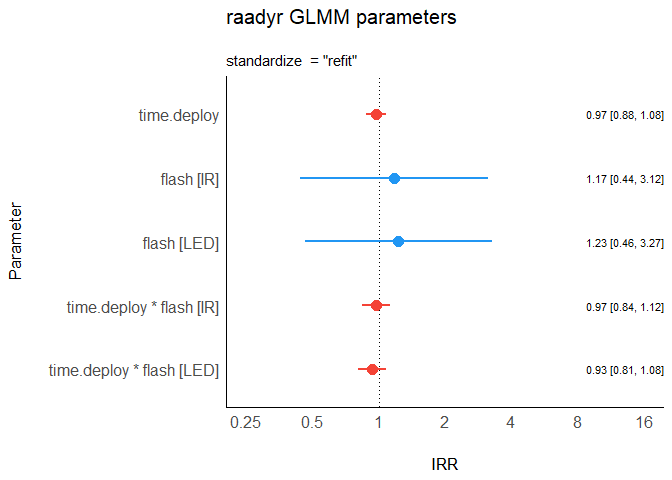
\includegraphics[scale=.4]{../R/glmm_sp_files/figure-gfm/parameters-2.png}
\caption{with values printed}
		\label{fig:para_raa2}
	\end{subfigure}
		\begin{subfigure}{.8\textwidth}
		  \centering
	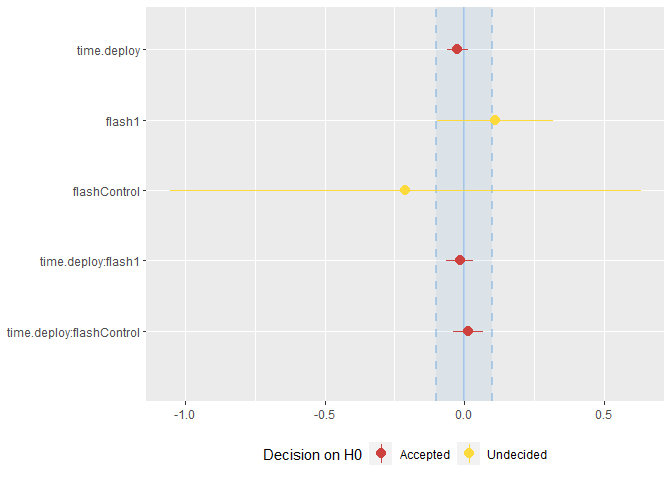
\includegraphics[scale=1]{../R/glmm_sp_files/figure-gfm/parameters-3.png}
\caption{Equivalence test}
		\label{fig:para_raa3}
	\end{subfigure}
		\caption{Visualising model parameters}
	\label{fig:para_sp}
\end{figure}



%\begin{figure}
%		  \centering
%		  	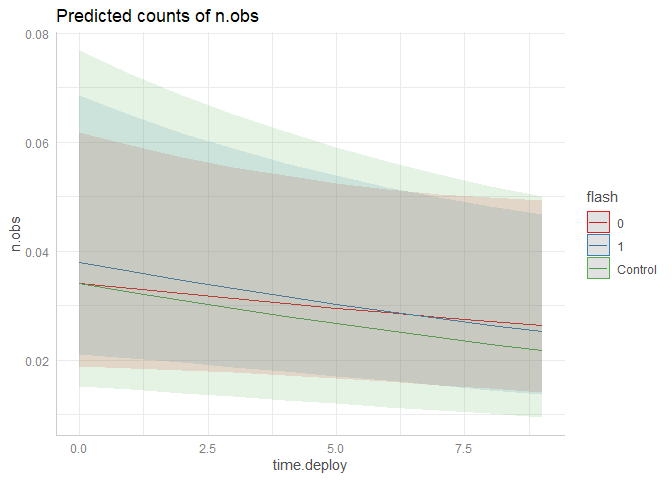
\includegraphics[width=.8\linewidth]{../R/glmm_sp_files/figure-gfm/raadyr-C-report-1.png}
%		  \caption{Roe deer}
%\end{figure}


\subsection{Equivalence test}

As all the parameters in the roe deer GLMM were considered non-significant, it is interesting to evaluate them against a Region of Practical Equivalence (ROPE) in an equivalence test.
When a parameter is within the ROPE in an equivalence test, it signifies that the difference from the mean, and the variance of the parameter, is low enough that we can accept H0 (that using white LED has no effect on the detection rate), rather than just fail to reject it.

According to this test, white LED is different enough that we cannot conclude on it’s immediate effect (intercept value), but it’s trend over time (interaction with time since deployment) is practically equivalent to H0. 
In other words, the equivalence test suggests that there is no significant difference in the long run, but there might be an increase in detections right after the day of deployment.
However, the increase could also result from inhereting a slightly higher detection rate from the IR periods \emph{if} there truly is a negative effect of the white LED over long periods of time.



%\subsection{CPH mixed effect}
%n.obs ~ time.deploy + flash*species + random.eff






